\documentclass[11pt]{article}

\usepackage[T1]{fontenc}
\usepackage{geometry}
\usepackage{amsmath, amssymb, amsthm}
\usepackage{listings}
% \usepackage{courier}
\usepackage{xcolor}
\usepackage{graphicx}
\usepackage{fancyhdr}
\usepackage{lipsum}
% \usepackage{subfigure}
\usepackage{caption}
\usepackage{subcaption}
\usepackage{float}
\usepackage{hyperref}

\makeatletter
\renewcommand\@biblabel[1]{}
\renewenvironment{thebibliography}[1]
     {\section*{\refname}%
      \@mkboth{\MakeUppercase\refname}{\MakeUppercase\refname}%
      \list{}%
           {\leftmargin0pt
            \@openbib@code
            \usecounter{enumiv}}%
      \sloppy
      \clubpenalty4000
      \@clubpenalty \clubpenalty
      \widowpenalty4000%
      \sfcode`\.\@m}
     {\def\@noitemerr
       {\@latex@warning{Empty `thebibliography' environment}}%
      \endlist}
\makeatother

% \captionsetup[table]{skip=10pt}

\geometry{a4paper, margin=1in, headheight=14pt}

\pagestyle{fancy}
\renewcommand\headrulewidth{0.4pt}
\fancyhead[L]{\scshape Experiment V}
% \lhead{Experiment I}
\rhead{}
\cfoot{\thepage}

\definecolor{darkgreen}{rgb}{0.2, 0.6, 0.4}
\definecolor{darkblue}{rgb}{0.2, 0.4, 0.8}
\lstset{ 
  basicstyle=\footnotesize\ttfamily,
  commentstyle=\color{gray},
  % extendedchars=true,
  % keepspaces=true,
  keywordstyle=\color{darkblue},
  % numbers=left,
  % numbersep=5pt,
  % numberstyle=\tiny\color{gray},
  stringstyle=\color{darkgreen},
  tabsize=4,
  % frame=lines,
  aboveskip=2em,
  belowskip=2em,
  breaklines=true
}

\newcommand\pp[2]{\frac{\partial #1}{\partial #2}}
\newcommand\E[1]{\langle #1 \rangle}

\title{
        \Large\textsc{PH2103: Physics Laboratory III} \\
        \vspace{10pt}
        \Huge \textbf{Quantum nature of atoms} \\
        \vspace{5pt}
        \large{Franck-Hertz experiment.}
}
\author{
        \large Satvik Saha%
        \thanks{Email: \tt ss19ms154@iiserkol.ac.in}
        \\\textsc{\small 19MS154}
}
\date{\normalsize
        \textit{Indian Institute of Science Education and Research, Kolkata, \\
        Mohanpur, West Bengal, 741246, India.} \\
        \vspace{10pt}
        \today
}

\begin{document}
        \maketitle

        % \renewcommand{\abstractname}{Aims}
        \begin{abstract}
                In this experiment, we demonstrate the quantum nature of atoms by performing the Franck-Hertz experiment
                using argon gas. Specifically, we show that electron bombardment can be used to excite atoms and the energy
                transferred during such interactions is quantized. Furthermore, the quantum of this energy transfer agrees with
                spectroscopic measurements of energy levels of argon.
        \end{abstract}

        \section{Theory}
        The Franck-Hertz experiment was set up to confirm certain predictions of the Bohr atomic model as well as previous spectroscopic results.
        It was found that atoms (of a particular element) emit and absorb radiation only at particular, discrete frequencies.
        This corresponds to discrete spectroscopic `lines' in the emission and absorption spectra of an atom.
        Using the relation $\Delta E = h\nu$, is is possible to create a ladder of corresponding discrete `energy levels' $E_n$, whereby any energy transfer
        is possible only if it corresponds to some $E_n - E_m$. In the Bohr model, energy transfers are explained in terms of the movements of 
        electrons between orbits/shells around the nucleus. These electrons are restricted to discrete radii/angular momenta, which
        lead to these dicrete energy levels. An electron moving from a higher to a lower energy level is accompanied by the release of
        the said difference in energy (typically as electromagnetic radiation), and vice versa.

        In this experiment, we verify these conclusions by considering a different sort of energy transfer, via inelastic collisions (scattering)
        with a beam of electrons. Suppose an electron is accelerated across a potential difference $U$, thus acquiring a momentum $p$.
        A vapour, say of argon, is kept in its path and the electron is collected by a plate on the other side.
        If this electron does not have sufficient kinetic energy to excite an argon atom, it can merely undergo elastic collisions with no energy transfer
        and is eventually collected on the other side -- with increasing applied potential, the collected current naturally increases.
        This is until the potential is sufficient to excite the argon atoms, i.e.\ is equal to the difference between two energy levels,
        say $\Delta E$. Now, the electrons undergo inelastic collisions, consequentially losing some momentum. If they are left with a
        momentum $p'$ at the end, we may conclude that $(p^2 - p'^2)/2m = \Delta E$.
        This means that at this threshold potential where $p' \approx 0$, i.e.\ $p^2 /2m\approx \Delta E$, the electrons are in effect immobilized
        by the argon vapour and do not make it to the collecting plate with sufficient energy, so the current drops sharply.
        This can be made more pronounced by imposing a negative potential in front of the collecting plate, so that only those electrons
        with a sufficiently high final momentum $p'$ are collected.
        Further increase in potential means that the current rises again, since the electrons have enough remaining momentum $p'$ even after one
        inelastic collision to make it to the other side, yet not enough to undergo a second inelastic collision.
        This is until the imparted kinetic energy $p^2 /2m \geq 2\Delta E$, whereby the electrons can undergo two inelastic collisions, 
        creating a second sharp drop in current. In this way, whenever $p^2 /2m \approx n\Delta E$, we observe a sharp drop in the collected 
        current before a subsequent rise.
        The potential difference between such drops is thus the excitation energy $\Delta E$. If the vapour is observed using a spectroscope,
        it can be seen that it emits light at a frequency precisely satisfying  $\Delta E = h\nu$. The wavelength associated with such light
        is $hc /\Delta E$.

        Recall that in the Bohr model, the energy levels of the orbits are given by
        \[
                E_n = -\frac{z^2}{n^2}R_E.
        \]
        Thus, in the case of argon ($z = 18$), the excitation corresponds to a transition from $n = 1 \to 2$. Hence, $\Delta E = -3 \times 18^2 R_E/4
        = 243 R_E$.
        We also use the relations for the energy, velocity and radius
        \[
                E_n = -\frac{1}{2}m v_n^2, \qquad mv_nr_n = n\hbar.
        \]

        Since the vapour used is kept at a very low pressure, the cathode current density may be described by the Richardson equation,
        \[
                j \propto T^2e^{-\phi /k_b T},
        \]
        where $\phi$ is the work function of the metal cathode and $T$ is the thermodynamic temperature.
        The space charge received by the anode is described by the Child-Langmuir Law,
        \[
                j = \frac{I}{A} = \sqrt{\frac{2e}{m_e}} \left(\frac{2\epsilon_0}{3d}\right)^2 V^{3 /2},
        \]
        where $A$ is the anode surface area, $d$ is the cathode-anode spacing, and $V$ is the anode voltage.
        Thus, when the electrons have the correct energy to undergo inelastic collisions, the anode current doesn't drop completely to zero.
        Instead, a proportion of electrons do indeed make it through without suffering collisions -- we thus expect the minima currents
        to follow the Child-Langmuir Law. Note that this law assumes ballistic motion with no scattering; this may not be the case at the 
        minima, since electrons may also suffer \textit{elastic} collisions and make it to the anode.
        
        \section{Experimental setup}
        A Franck-Hertz apparatus is set up, which is simply a tetrode filled with argon vapour.
        The discharge tube and plates are set up as in Fig.~\ref{fig:FH}.
        Electrons are produced by a heated cathode $K$ and are accelerated between two grids $G_1$ and $G_2$ by a potential
        difference $V$ across $G_2K$. A negative potential is also applied across $G_2A$ so as to prevent electrons below
        a threshold energy from passing. The current collected at the anode $A$ is recorded as a function of $V$.

        \begin{figure}[h]
                \centering
                \includegraphics[width=0.6\textwidth]{./FH.png}
                \caption{A circuit diagram of the Franck-Hertz experiment.}
                \label{fig:FH}
        \end{figure}
        
        
        \section{Experimental data and analysis}
        
        \subsection{Processing and plotting}
        
        All data has been gathered into an Excel spreadsheet, read using \texttt{pandas} and processed using \texttt{numpy}.
        The locations of the minima were recorded using the coordinate tool from \texttt{pyplot}.
        The code used has been listed below.

        \lstinputlisting[language=Python]{plot.py}

        The current vs applied voltage profile has been presented in Fig.~\ref{fig:VI}.
        \begin{figure}[h]
                \centering
                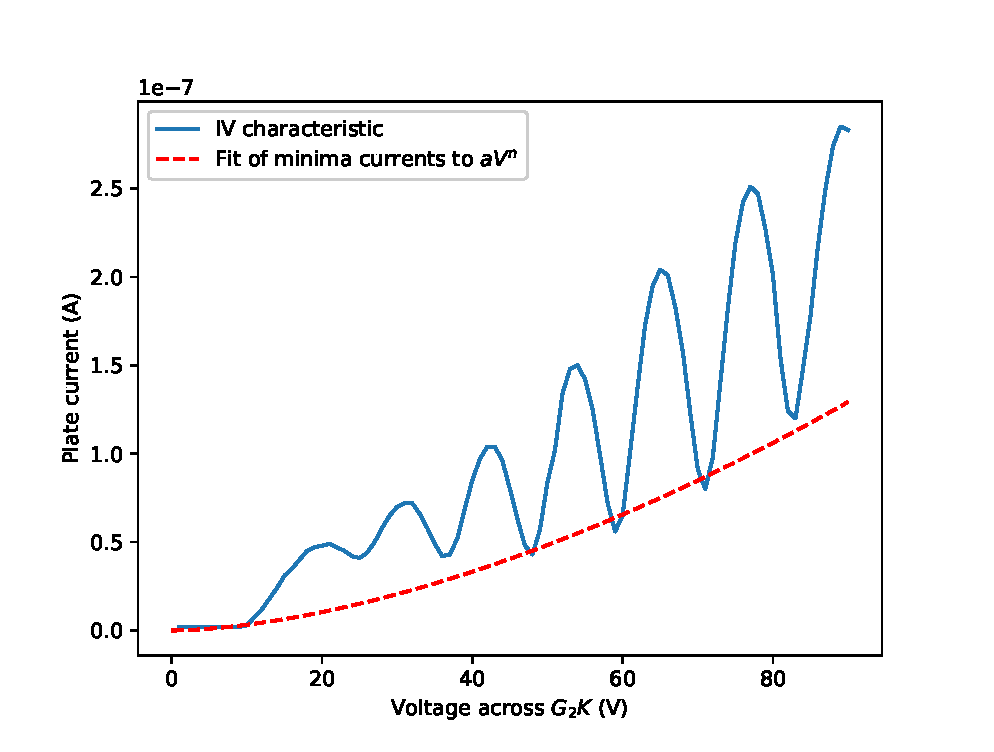
\includegraphics[width=\textwidth]{./VI.eps}
                \caption{The captured electron beam current vs accelerating voltage profile shows periodic dips at intervals of around 11-12 V.
                The minima currents have been fitted to the equation $I = aV^n$. We obtain $n = 1.67 \pm 0.32$ and $a \approx 7\times 10^{-11}$.}
                \label{fig:VI}
        \end{figure}

        We record the positions of the minima, with the corresponding potential differences in Table~\ref{tab:diff}.
        \begin{table}[H]
                \centering
                \caption{Positions of minima in the current-voltage profile and the corresponding peak separations.}
                \label{tab:diff}
                \begin{tabular}{ccc}\hline
                Position of peak (V)    &       Difference (V)  &       Current ($10^{-7}$ A)       \\\hline\hline
                        25.0            &                       &       0.41    \\
                                        &       11.5            &               \\
                        36.5            &                       &       0.42    \\
                                        &       11.5            &               \\
                        48.0            &                       &       0.43    \\
                                        &       11.0            &               \\
                        59.0            &                       &       0.56    \\
                                        &       12.0            &               \\
                        71.0            &                       &       0.80    \\
                                        &       12.0            &               \\
                        83.0            &                       &       1.20    \\\hline
                        Mean            &       11.6            &               \\\hline
                \end{tabular}
        \end{table}

        Thus, we see that $\Delta E \approx 11.6$ eV $\approx 1.86\times 10^{-18}$ J, where the excitation is between the energy levels $1$ and $2$.
        We use this to calculate
        \[
                R_E = \frac{\Delta E}{243}, \qquad E_1 = -z^2 R_E = -\frac{324}{243}\Delta E = -15.47 \text{ eV}.
        \]
        This is the first ionization energy of argon. The literature value is $-15.76$ eV.
        We thus calculate the velocity and radius of the elctron in the first orbit,
        \[
                v_1 = \sqrt{\frac{2E_1}{m}} = 2.33\times 10^{6} \text{ m/s}, \qquad r_1 = \frac{\hbar}{mv_1} = 4.96\times 10^{-11}\text{ m} \approx
                        49.6 \text{ pm}.
        \]
        The literature value for the $s$ shell radius is around $62.5$ pm\footnote{\url{https://www.webelements.com/argon/atom_sizes.html}}
        however, with the total radius of the (non-bonded) argon atom being around $3r_1 = 188$ pm\footnote{
        \url{https://www.rsc.org/periodic-table/element/18/argon}}.

        \subsection{Error Analysis}
        While recording the extrema positions, we estimate an uncertainty of $\delta V \approx 1$ V.
        Thus, the erorr in the difference is given by $\delta U = \sqrt{2}\delta V \approx 1.4$ V.
        Since we have made 5 such measurements of the difference, our error is cut down by a factor of $\sqrt{5}$.
        Thus, the uncertainty in our mean is $\delta E \approx 0.6$ V.
        
        We can use the standard error propagation formulae to obtain
        \[
                \delta E_1 = \frac{324}{243}\delta(\Delta E) = 0.8\text{ eV}.
        \]
        The error from the standard literature value of $-15.76$ eV is $1.8\%$.
        Also,
        \[
                \delta v = \left|\frac{\partial v}{\partial E}\right|\delta E = \frac{1}{2}E^{-1 /2}\sqrt{\frac{2}{m}}\,\delta E,\qquad
                \delta v_1 = \frac{v_1}{2}\frac{\delta E_1}{E_1} = 0.06\times 10^6 \text{ m/s}.
        \]
        Furthermore,
        \[
                \delta r = \left|\frac{\partial r}{v}\right|\delta v = \frac{\hbar}{mv^2}\delta v, \qquad
                \delta r_1 = r_1\frac{\delta v}{v} = 1.3\text{ pm}.
        \]
        The error from the literature value of $62.5$ pm is incredibly high, around $20\%$.
        This strongly indicates that the Bohr model is not suitable for such calculations involving multi-electron systems,
        without severe corrections for the interactions between the electrons.


        \subsection{Reported Values}
        We report a minima separation of $11.6 \pm 0.6$ V. This agrees with measurements of spectral lines of argon, specifically
        one at $104.8$ nm, which corresponds to an energy of $11.83$ V.
        Our measurement differs from this by $3.6\%$.

        The calculated first ionization of argon is $-15.46 \pm 0.8$ eV, which also agrees with the literature value of $-15.76$ eV.
        The calculated Bohr radius of the first shell $49.6 \pm 1.3$ pm is wildly off the expected value of $62.5$ pm.

        \section{Discussion}
        We note that the choice of argon instead of mercury has been made since it is fairly inert and non-toxic.

        We have seen that the Bohr model has been validated in terms of the discretisation of energy levels, and the 
        calculated excitation and ionization energies agree well with literature values. On the other hand, the Bohr model
        does not hold up structurally, for example during calculations of orbital radii. These require more sophisticated
        corrections, especially in multi-electron systems. The Schr\"odinger equation may be invoked to obtain more accurate results.

        It may also be noted that the minima currents loosely seem to follow the Child-Langmuir Law, as seen in Fig.~\ref{fig:VI}.
        The fit $I \propto V^n$ yielded $n = 1.67 \pm 0.32$, which agrees with the $3 /2$ power law.
        Note that the fit is very poor, especially at the lower potentials where the minima currents seem constant.

        \subsection{Sources of error}

        Errors may be introduced by fluctuations of potentials across the plates or impurities in the vapour used.

        The discrepancy between the minima currents and the Child-Langmuir Law may be explained by the fact that the assumptions
        are not fully satisfied -- electrons may indeed be scattered and do not always follow ballistic motion. However,
        with increasing potential, the tendency of these electrons to undergo such elastic collisions decreases, and
        thus the latter half of the minima currents fit well with the $3 /2$ power law.
        
        \section{Conclusion}
        In conclusion, we have demonstrated that the energy transferred to atoms during inelastic electron collisions is indeed
        quantized, in accordance with the quantization of emitted and absorbed electromagnetic radiation as seen from spectroscopy.
        This validates Bohr's model of electron energy levels in atoms.

        % \nocite{*}
        % \bibliographystyle{plain}
        % \bibliography{ref}

\end{document}
